%% ==============================
\chapter{Results}
\label{sec:results}
%% ==============================
The results of this work are the straight path planner ILIR, the hierarchical planning algorithm, and the planner plugin for integration into ROS 2. In this chapter, these approaches are evaluated and compared with related work. The evaluation criteria have been presented in Chapter \ref{sec:methods} "Methods".

%% ==============================
\section{Comparison of Straight Path Planners}
\label{sec:evaluation_straight_path}
%% ==============================
The evaluation of the planner algorithm ILIR is done on the benchmark maps of Ryu \cite{ryu_hierarchical_2020} and Hou et al. \cite{hou_straight_2021}. And to specifically show the effects of public space disturbance, the second room of the first map and the ninth room of the second map were chosen. The metrics and the calculation of the number of paths used on each map were presented in Chapter \ref{sec:methods}. For better readability, a complete list is repeated here:

\begin{enumerate}
    \item \textbf{Success Rate}: Percentage of valid paths found
    \item \textbf{Path Length}: Total length from start to goal in pixels
    \item \textbf{Planning Time}: Total planning time including smoothing
    \item \textbf{Path Smoothness}: Sum of deviation angles divided by path length
    \item \textbf{Obstacle Clearance}: Mean distance from path to obstacles
    \item \textbf{Distance Deviation}: Standard deviation of distance between path and obstacles
    \item \textbf{Distance to Centroid}: Mean distance of the path to the centroid of the room
    \item \textbf{Disturbance of Public Space}: Largest open area within the map divided by total room area (details in Chapter \ref{sec:new_metric})
\end{enumerate}

The different planners that will be compared to the ILIR algorithm are listed below. These planners were chosen because they are widely used in the field of path planning for robotics and provide a good baseline for comparison. In addition, A* can be considered the ground truth for the shortest path distance since it is complete and optimal. The other two represent the different approach of probabilistic sampling.

\begin{enumerate}
    \item \textbf{ILIR}: Iterative Largest Interior Rectangle
    \item \textbf{A*}: A* Planner
    \item \textbf{PRM}: Probabilistic Roadmap
    \item \textbf{RRT}: Rapidly Exploring Random Tree
\end{enumerate}

\begin{figure}[h]
    \captionsetup[subfigure]{justification=centering}
    \centering
    \begin{subfigure}{.25\textwidth}
      \centering
      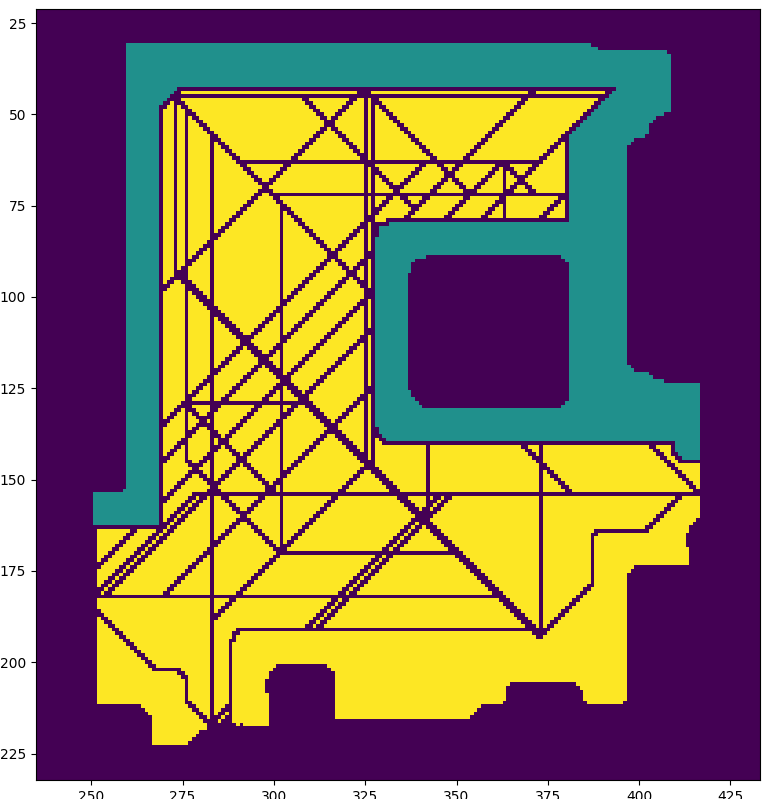
\includegraphics[width=\textwidth]{figures/60_results/room2_disturbance_astar_unsmoothed.png}
      \caption{A*}
    \end{subfigure}%
    \begin{subfigure}{.24\textwidth}
      \centering
      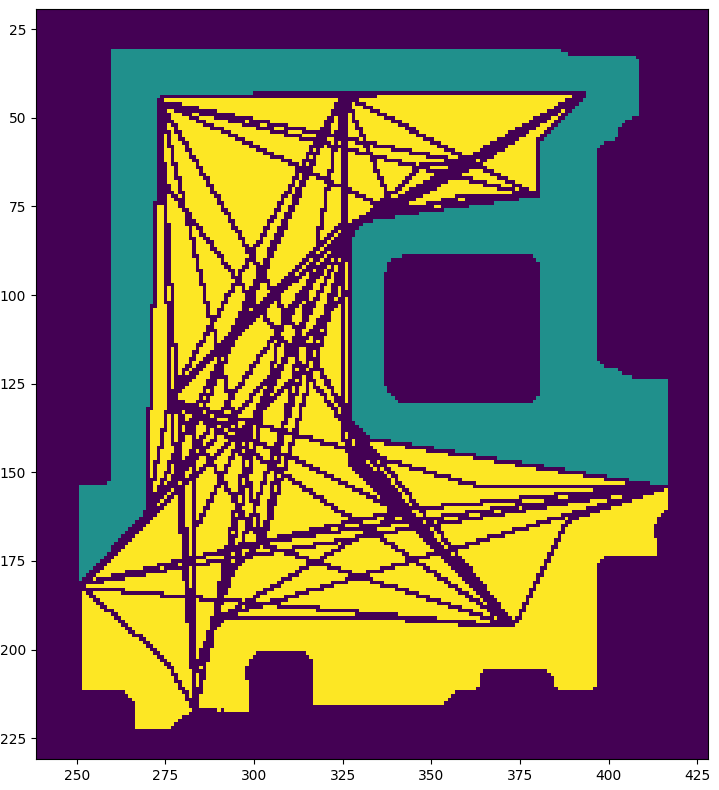
\includegraphics[width=\textwidth]{figures/60_results/room2_disturbance_astar_smooth.png}
      \caption{A* smoothed}
    \end{subfigure}
    \caption[Comparison of A* with and without smoothing algorithm]{Comparison of A* with and without smoothing algorithm. Turquoise and yellow areas are both representing the original room map.}
    \label{fig:smoothing}
\end{figure}

The first step for a fair comparison is to smooth the output path of each planner as it would realistically be used by a robot for driving. This is necessary because the A*, for example, produces paths on a gridmap that has a certain resolution. This leads to "steps" for diagonal lines. And there are always many possible solution paths with exactly the same length. It is only determined by the order of node expansion by the specific implementation. To force the path to take the most direct route, unnecessary nodes are removed and the more direct connection is chosen. Figure \ref{fig:smoothing} shows the effect of this smoothing. The same is done for PRM and RRT. Both planners create a roadmap by sampling random points in the environment. This roadmap is then connected and provides a path. This is not optimal because there are many unnecessary turns. For smoothing, the nodes with the highest deviation angles between the incoming and outgoing lines are tried to be removed. If this is possible, the surrounding nodes are connected directly and the process is repeated until no node can be removed because it would result in a collision path. This is not done for the ILIR, because it would contradict the goal of leaving the middle for undisturbed human traffic.

\begin{figure}[h]
    \captionsetup[subfigure]{justification=centering}
    \centering
    \begin{subfigure}{.25\textwidth}
      \centering
      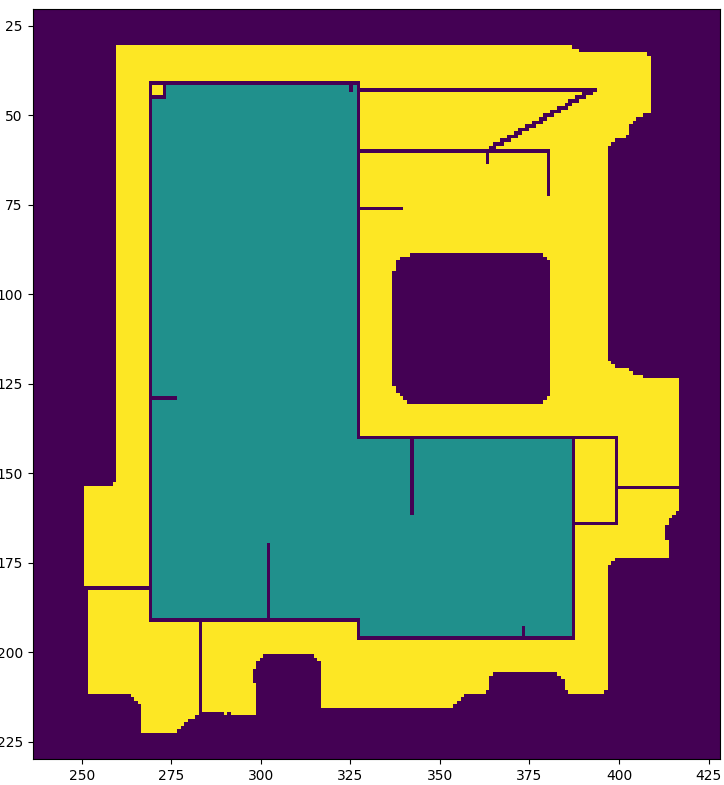
\includegraphics[width=\textwidth]{figures/60_results/room2_disturbance_ilir.png}
      \caption{ILIR}
    \end{subfigure}%
    \begin{subfigure}{.25\textwidth}
      \centering
      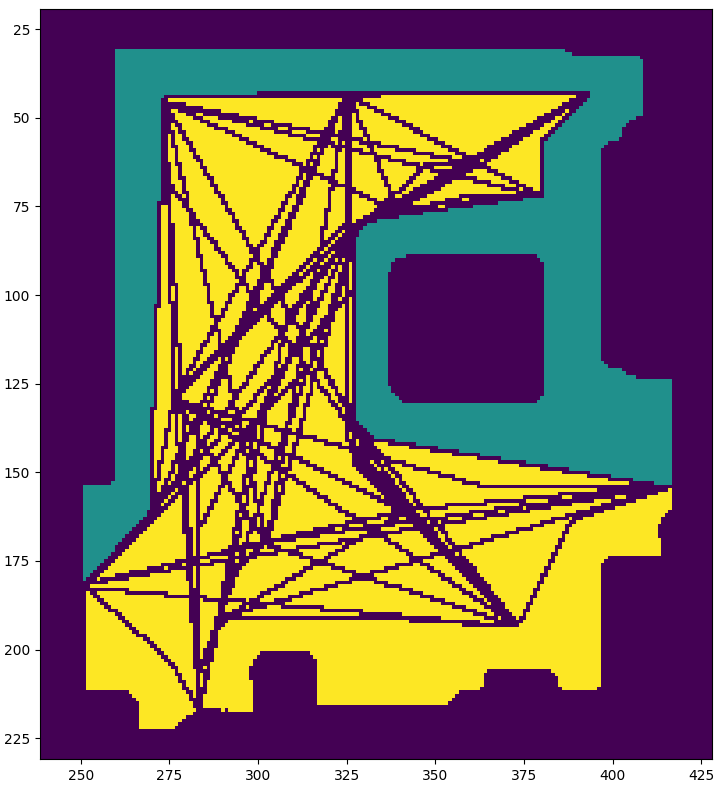
\includegraphics[width=\textwidth]{figures/60_results/room2_disturbance_astar.png}
      \caption{A*}
    \end{subfigure}%
    \begin{subfigure}{.25\textwidth}
      \centering
      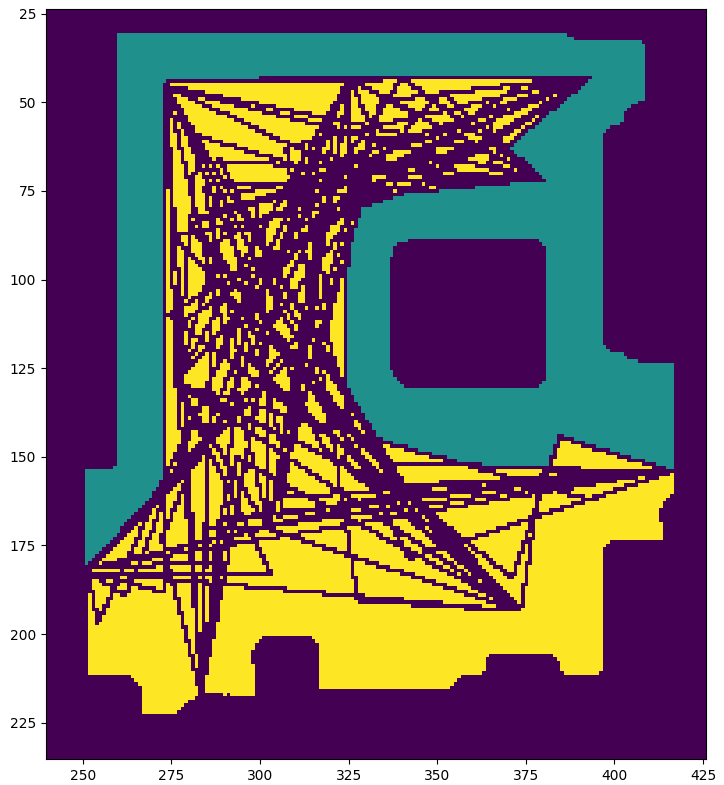
\includegraphics[width=\textwidth]{figures/60_results/room2_disturbance_prm.png}
      \caption{PRM}
    \end{subfigure}%
    \begin{subfigure}{.25\textwidth}
      \centering
      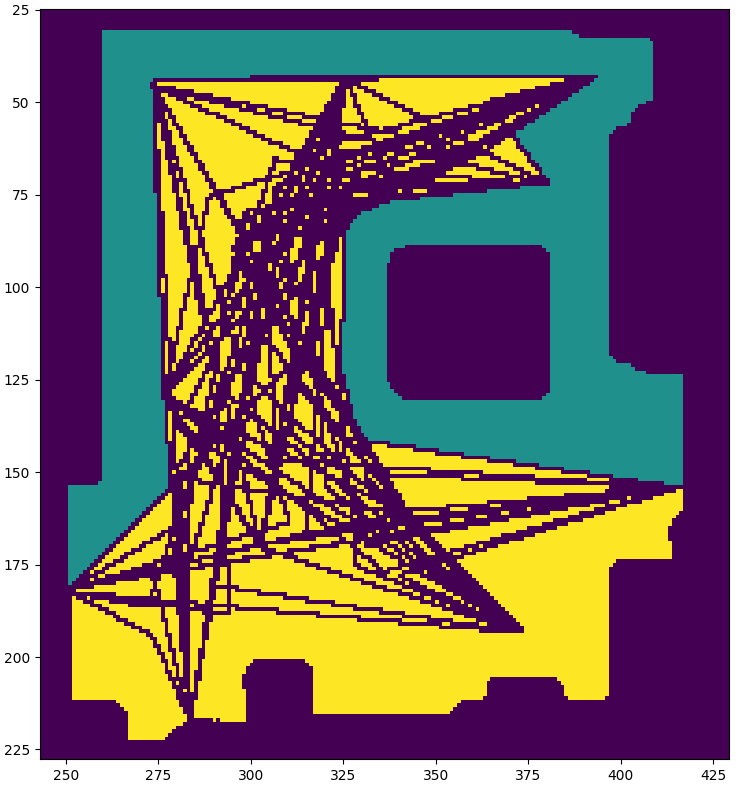
\includegraphics[width=\textwidth]{figures/60_results/room2_disturbance_rrt.png}
      \caption{RRT}
    \end{subfigure}
    \caption[Comparison of planning methods on room 2 of benchmark map 1]{Comparison of planning methods on room 2 of benchmark map 1 with 78 paths. The turquoise area is the largest free area where no path is crossing and the combination with yellow is the original room map.}
    \label{fig:ryu_room2_comparison}
\end{figure}

Figure \ref{fig:ryu_room2_comparison} shows the comparison of smoothed paths in the second room of the first benchmark map. It can be clearly seen that the ILIR planner forces the paths onto its roadmap and keeps the inner area free. In the figure, the metric for public space disturbance is represented visually by the colors of the background: the turquoise area is the largest free area where no path crosses, and the remaining area is yellow. The calculation of this metric is explained in Chapter \ref{sec:methods} with the formula \ref{equ:disturbance}.

\begin{table}[ht]
\centering
\begin{tabular}{lc|cccc}
\hline
\textbf{Metric} & \textbf{Unit} & \textbf{ILIR} & \textbf{A*} & \textbf{PRM} & \textbf{RRT} \\
\hline
Success rate & -                & \textbf{1.000}          & \textbf{1.000}          & \textbf{1.000}      & 0.987 \\
Mean planning time & s          & \textbf{0.002} & 1.094         & 0.879     & 0.014 \\
Mean path length & px           & 204.4          & \textbf{118.8} & 136.3    & 131.5 \\
Mean smoothness & °/px          & 1.296         & \textbf{0.203} & 0.241    & 0.214 \\
Mean obstacle clearance & px    & \textbf{14.4} & 22.5          & 25.4      & 25.4 \\
Std obstacle clearance & px     & \textbf{4.1}  & 5.9           & 5.7       & 5.9 \\
Mean distance to centroid & px  & \textbf{70.0}          & 56.6          & 57.7      & 56.3 \\
Disturbance of public space & - & \textbf{0.443} & 0.698          & 0.663      & 0.664 \\
\hline
\end{tabular}
\caption{Comparison of planning methods on room 2 of benchmark map 1 with 78 paths}
\label{tab:room2_results}
\end{table}

Table \ref{tab:room2_results} shows the results of the evaluation for each planner. The room 2 represents an average room that could appear on most floors in an office environment. It is only about ~8x6 m in size. But already in this small room the differences between the planners are visible. Due to its geometrically built roadmap compared to expanding single nodes over the entire coordinate space, ILIR is the fastest with 2 ms, followed by RRT with 14 ms. This is an improvement of 86 \%. Note that the ILIR's roadmap creation time occurs during the room segmentation and is not included here. In terms of path length, as expected, the A* planner has the shortest path and ILIR has the longest since it avoids the middle area. The smoothness is a factor that is surprisingly bad for ILIR with 2.37 °/px. It was expected that by forcing straight paths the resulting path would be smoother. But this is a false conclusion, as it has more 90° turns than the others. This adds up to a large total turn angle and cannot be compensated by the longer path. The obstacle clearance of ILIR is low, which is not necessarily a bad thing as it shows that the paths are closer to the wall. The standard deviation of this distance shows that these paths are also more consistent than the others. The metric of the distance to the centroid of the room also shows that the paths of ILIR do not go directly through the center. This means that the paths are close to the walls and are generally less fluctuating than the paths of the other planners. Finally, the custom metric for the disturbance of the room space shows that ILIR has the lowest disturbance with 44.3 \%, which is 22 \%-points better than the next best. This proves that the ILIR planner achieves its goal of planning paths that are straight and do not disturb the human working area even in a small room. Also in Figure \ref{fig:ryu_room2_comparison} it can be clearly seen that the paths are deterministic and always follow the same roadmap. This makes them more predictable for humans.

\begin{figure}[h]
    \captionsetup[subfigure]{justification=centering}
    \centering
    \begin{subfigure}{.35\textwidth}
      \centering
      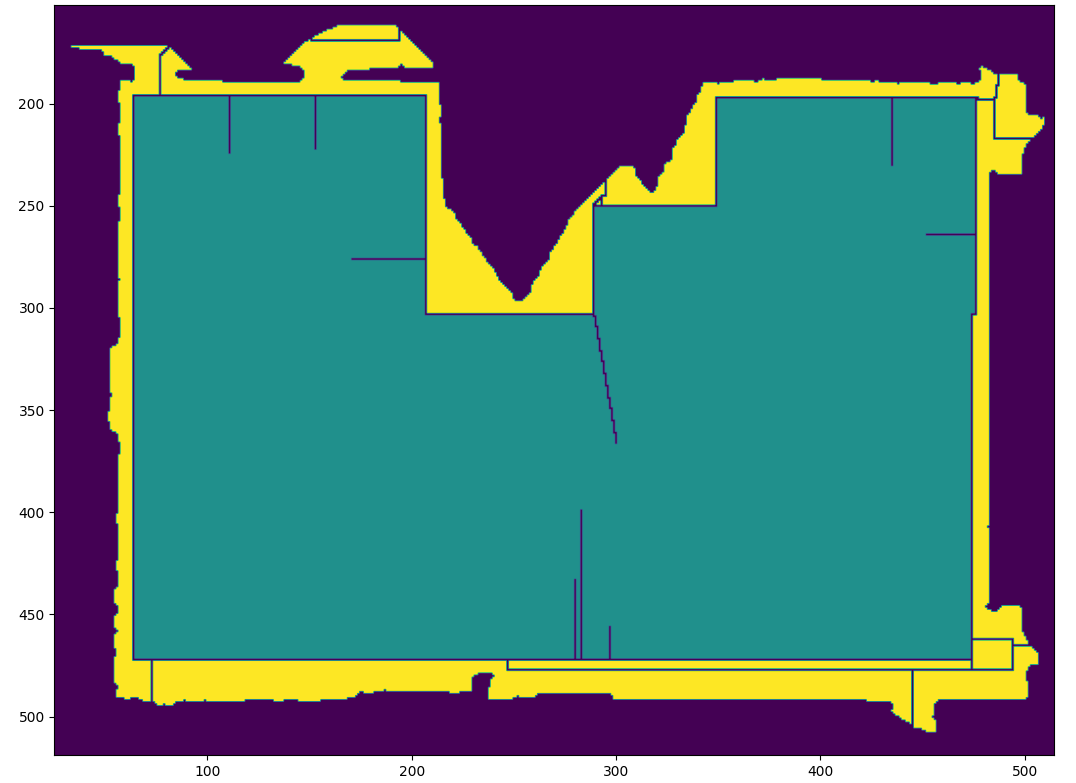
\includegraphics[width=\textwidth]{figures/60_results/room9_disturbance_ilir.png}
      \caption{ILIR}
    \end{subfigure}%
    \begin{subfigure}{.35\textwidth}
      \centering
      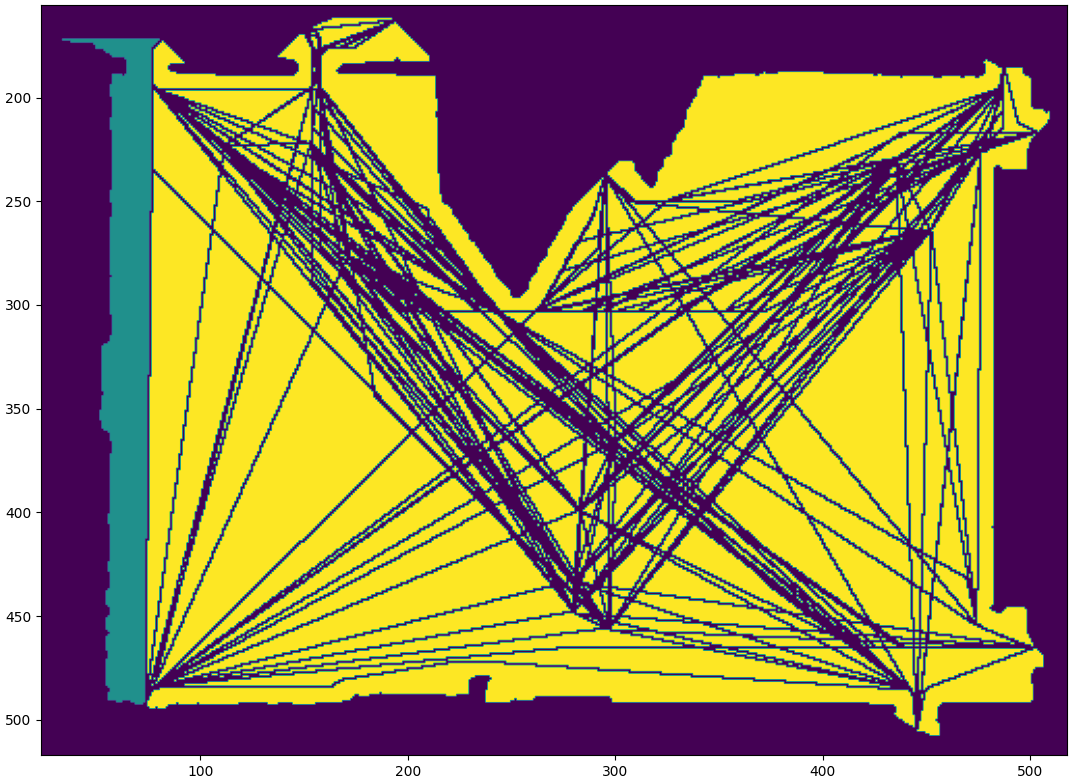
\includegraphics[width=\textwidth]{figures/60_results/room9_disturbance_astar.png}
      \caption{A*}
    \end{subfigure}
    \begin{subfigure}{.35\textwidth}
      \centering
      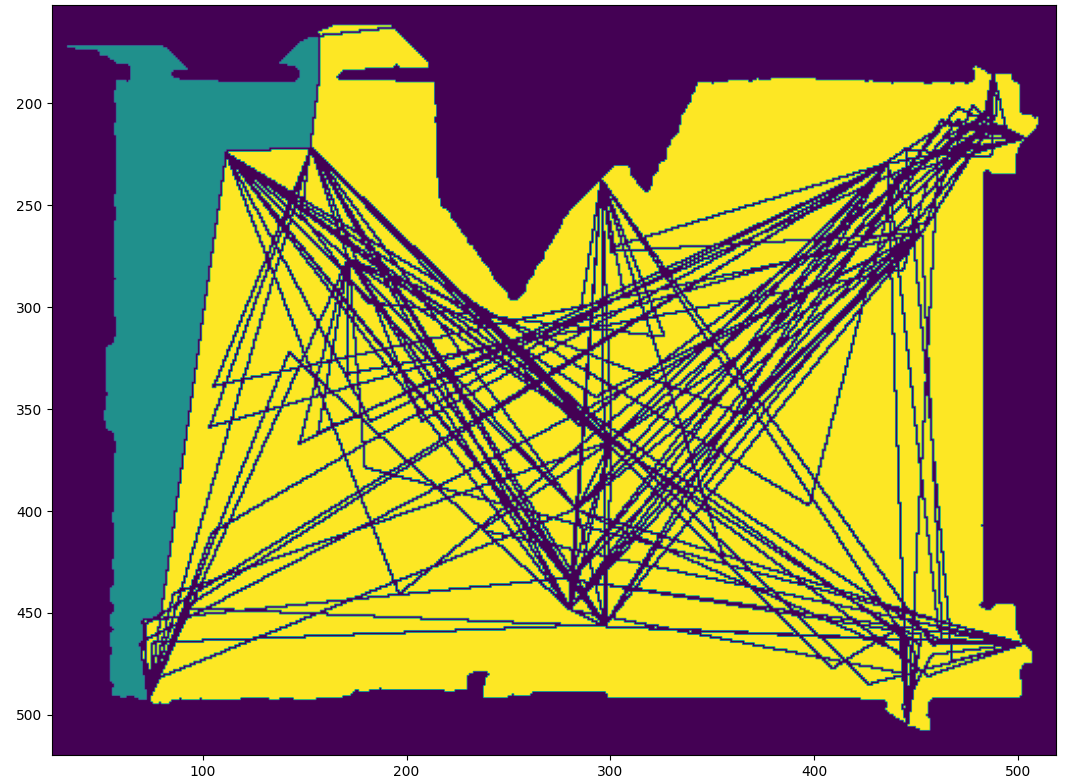
\includegraphics[width=\textwidth]{figures/60_results/room9_disturbance_prm.png}
      \caption{PRM}
    \end{subfigure}%
    \begin{subfigure}{.35\textwidth}
      \centering
      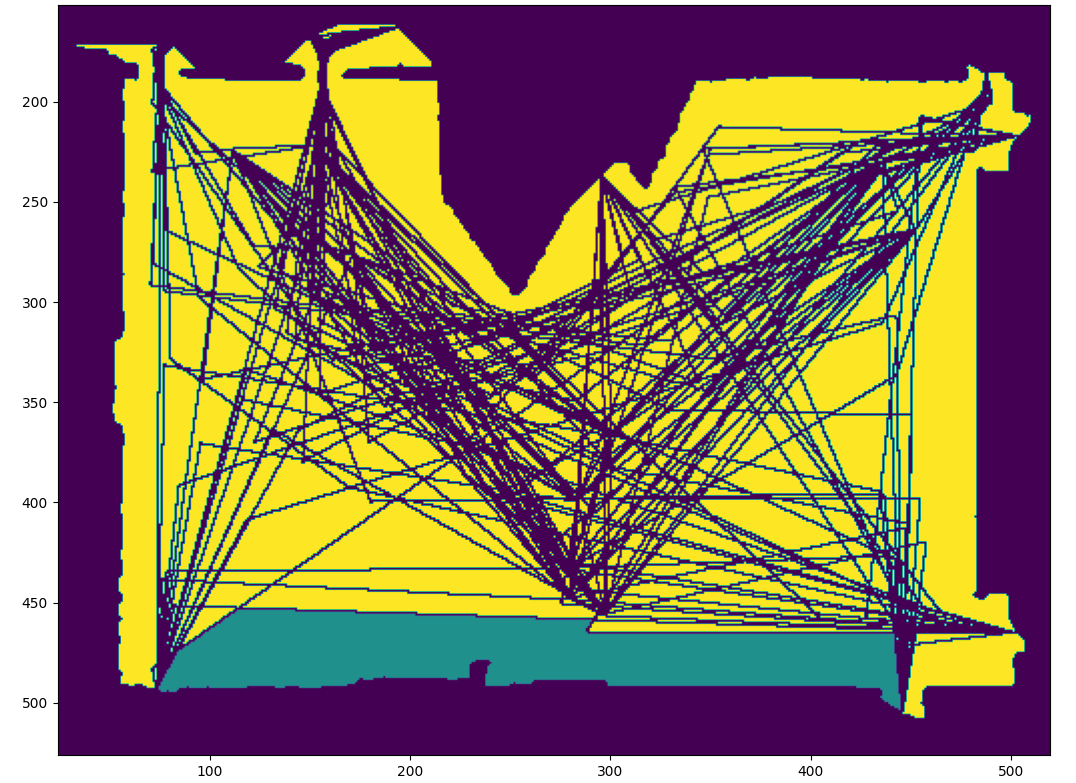
\includegraphics[width=\textwidth]{figures/60_results/room9_disturbance_rrt.png}
      \caption{RRT}
    \end{subfigure}
    \caption[Comparison with common planners on room 9 of benchmark map 2]{Comparison with common planners on room 9 of benchmark map 2 with 171 paths. The turquoise area is the largest free area where no path is crossing and the combination with yellow is the original room map.}
    \label{fig:hou_room9_comparison}
\end{figure}

\begin{table}[h]
\centering
\caption{Comparison of planning methods on room 9 of benchmark map 2 with 171 paths}
\label{tab:room9_results}
\begin{tabular}{lc|cccc}
\hline
\textbf{Metric}                    & \textbf{Unit} & \textbf{ILIR} & \textbf{AStar} & \textbf{PRM} & \textbf{RRT} \\
\hline
Success rate                       & -    & \textbf{1.000}          & \textbf{1.000}         & 0.632          & 0.942 \\
Mean planning time                 & s    & \textbf{0.141} & 8.077         & 0.962          & 0.783 \\
Mean path length                   & px   & 496.3          & \textbf{256.8}& 262.0          & 304.6 \\
Mean smoothness                    & °/px & 1.374          & 0.248         & \textbf{0.205} & 0.245 \\
Mean obstacle clearance            & px   & \textbf{15.2}  & 45.0          & 53.5           & 53.1  \\
Std obstacle clearance             & px   & \textbf{9.1}   & 17.6          & 18.0           & 19.9 \\
Mean distance to centroid          & px   & \textbf{175.7}          & 134.6         & 126.3          & 128.9  \\
Disturbance of public space        & -    & \textbf{0.166} & 0.951         & 0.921          & 0.887 \\
\hline
\end{tabular}
\end{table}

For comparison, the same metrics are now applied to a conference lobby that is much larger (~30x50 m) and has more entrances. Figure \ref{fig:hou_room9_comparison} shows this room. The corresponding result of the evaluation is shown in Table \ref{tab:room9_results}. For this benchmark, the ILIR planner is again the fastest in terms of planning time with 0.141 s per path. The mean obstacle clearance, its standard deviation, and the distance to the centroid again show that ILIR's paths are closer to the walls and less fluctuating. The difference in the disturbance of the public space is even greater, and with more than 72 \%-points apart and a total of 16 \% of the room area occupied by potential paths of the robot, it leaves enough space for human activities.

In the previous evaluation, some rooms were highlighted to demonstrate the planner's capabilities on an average map as well as for an extreme case. But of course most of the robot's paths are through corridors. Especially there the goal property of straight paths is important to avoid collisions with people and to establish a predictable behavior. For this reason, the focus of the following evaluation is on the straight paths and the general appearance, and not on the path-specific metrics. 

\begin{figure}[h]
    \captionsetup[subfigure]{justification=centering}
    \centering
    \begin{subfigure}{.5\textwidth}
      \centering
      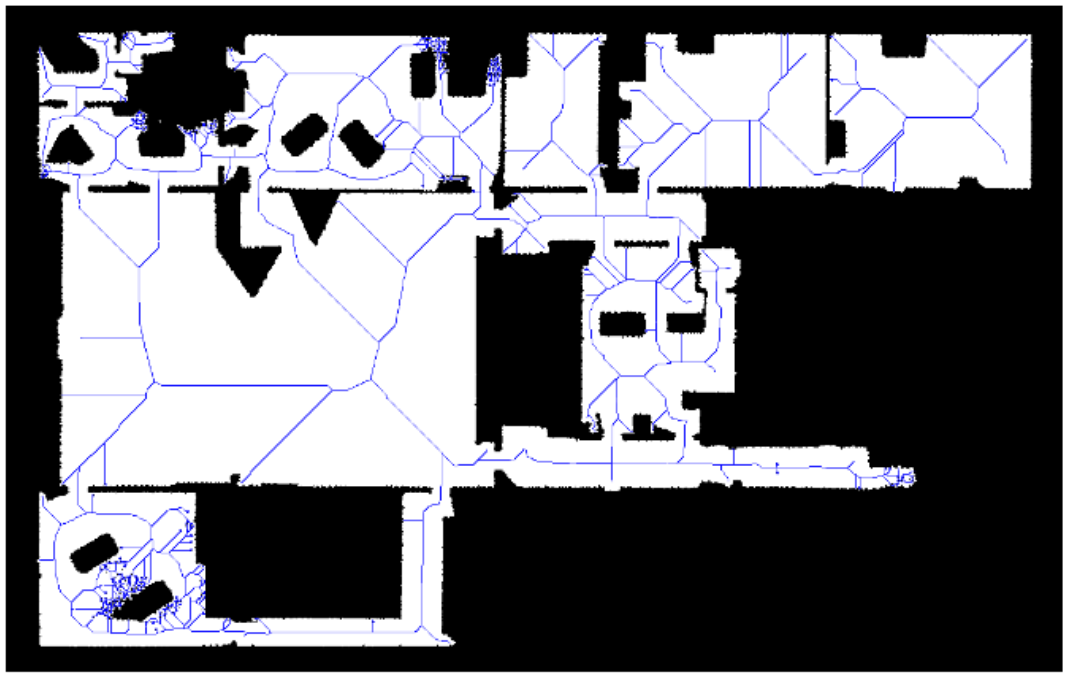
\includegraphics[width=\textwidth]{figures/60_results/hou2_roadmap_RGVG.png}
      \caption{RGVG \cite{beeson_towards_2005}}
    \end{subfigure}%
    \begin{subfigure}{.5\textwidth}
      \centering
      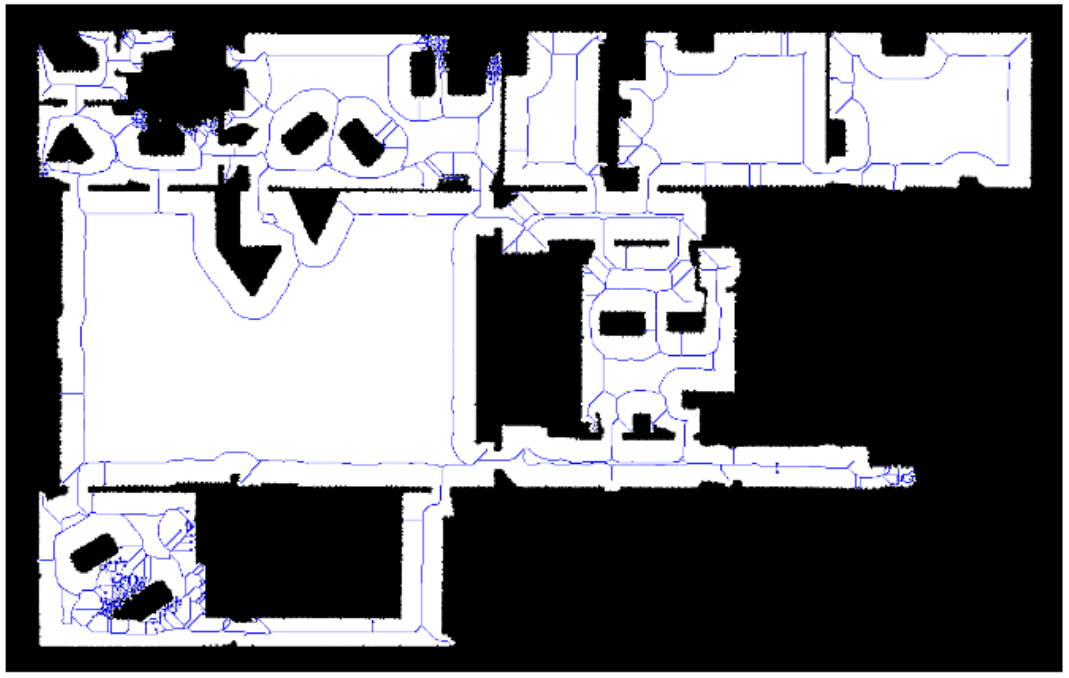
\includegraphics[width=\textwidth]{figures/60_results/hou2_roadmap_evg.png}
      \caption{EVG \cite{beeson_towards_2005}}
    \end{subfigure}
    \begin{subfigure}{.5\textwidth}
      \centering
      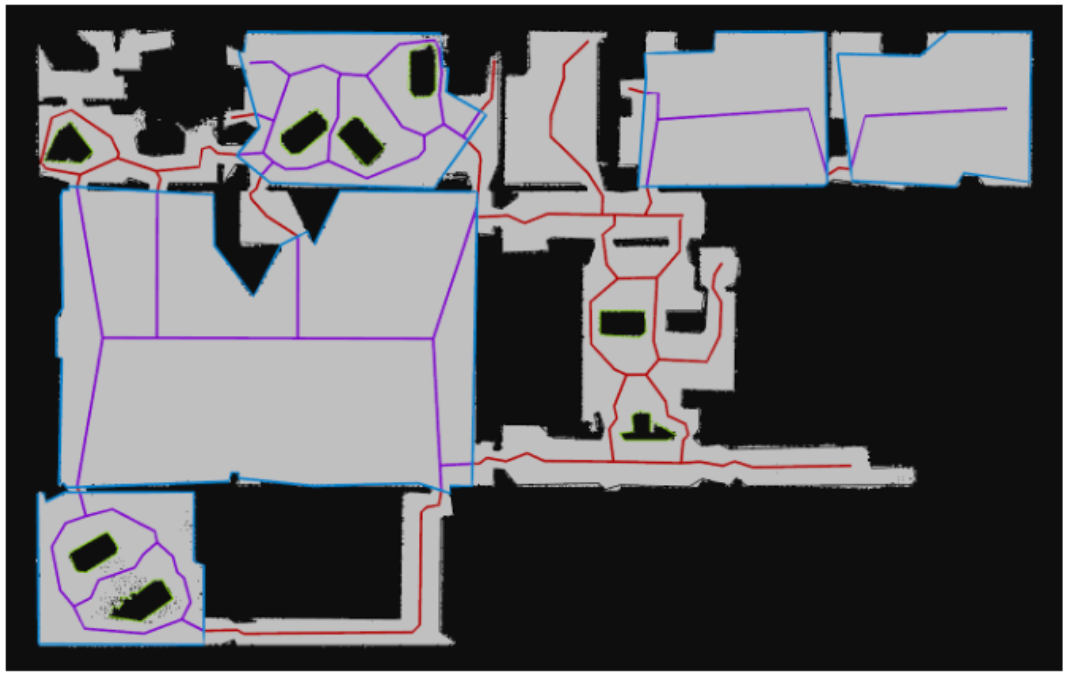
\includegraphics[width=\textwidth]{figures/60_results/hou2_roadmap_htm.png}
      \caption{HTM \cite{hou_straight_2021}}
    \end{subfigure}%
    \begin{subfigure}{.5\textwidth}
      \centering
      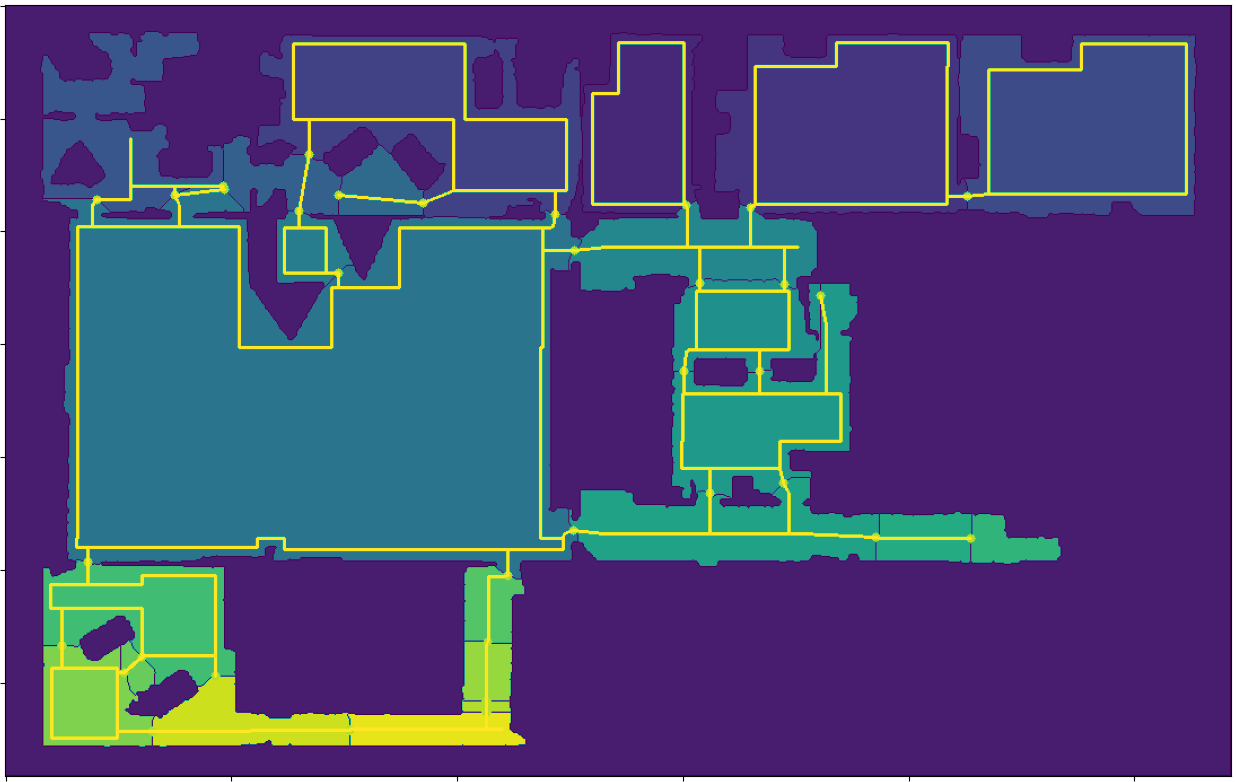
\includegraphics[width=\textwidth]{figures/60_results/hou2_roadmap_ilir.png}
      \caption{ILIR}
    \end{subfigure}
    \caption[Comparison with related work on room 9 of benchmark map 2]{Comparison with related work on room 9 of benchmark map 2. The roadmap is drawn in blue, red and yellow, obstacles are black and dark purple}
    \label{fig:hou_comparison}
\end{figure}

Figure \ref{fig:hou_comparison} shows the complete benchmark map 2 and the roadmaps generated by the Reduced General Voronoi Graph (RGVG), the Extended Voronoi Graph (EVG) \cite{beeson_towards_2005}, the Hierarchical Topological Map (HTM) \cite{hou_straight_2021} and the ILIR planner (this work). It can be seen that the EVG in \ref{fig:hou_comparison} (b), which is configured with a sensory horizon of 1.5 m, always stays close to the wall if there is a larger room. If not, it stays in the middle of the corridor. However, it suffers from strong jitter caused by sensor noise. The paths in the corridor are not straight and not good for driving a robot. The HTM approach (c) solves the straight path problem for the corridor well, but struggles in larger rooms. The paths are straight but almost never parallel to the walls and go straight through the open space. The ILIR planner (d) solves both problems by providing straight paths in the middle of each corridor, while staying close and parallel to the walls in large open areas. Since the implementations of the other approaches are not open source, it was not possible to directly compare these paths with specific metrics.

%% ==============================
\section{Comparison of Hierarchical Planners}
\label{sec:evaluation_hierarchical}
%% ==============================
The hierarchical planner should be compared to other implementations from related work using a common set of benchmarks. Since such a common set of benchmarks does not exist, and the planners from related work are not open source, this evaluation for the entire n-level H-Graph is done only as a proof of concept. However, the SIRRT* algorithm by Ryu \cite{ryu_hierarchical_2020} uses the same benchmark map 1 and also implements a hierarchical planner, although only for two levels of hierarchy. Figure \ref{fig:ryu_floor_comparison} shows a comparison between SIRRT* and the proposed hierarchical planner combined with the roadmap from ILIR. Note that the SIRRT* planner is limited to two levels of hierarchy, as its focus is only on improving the speed of calculating paths in huge floors. 

\begin{figure}[h]
    \captionsetup[subfigure]{justification=centering}
    \centering
    \begin{subfigure}{0.75\textwidth}
      \centering
      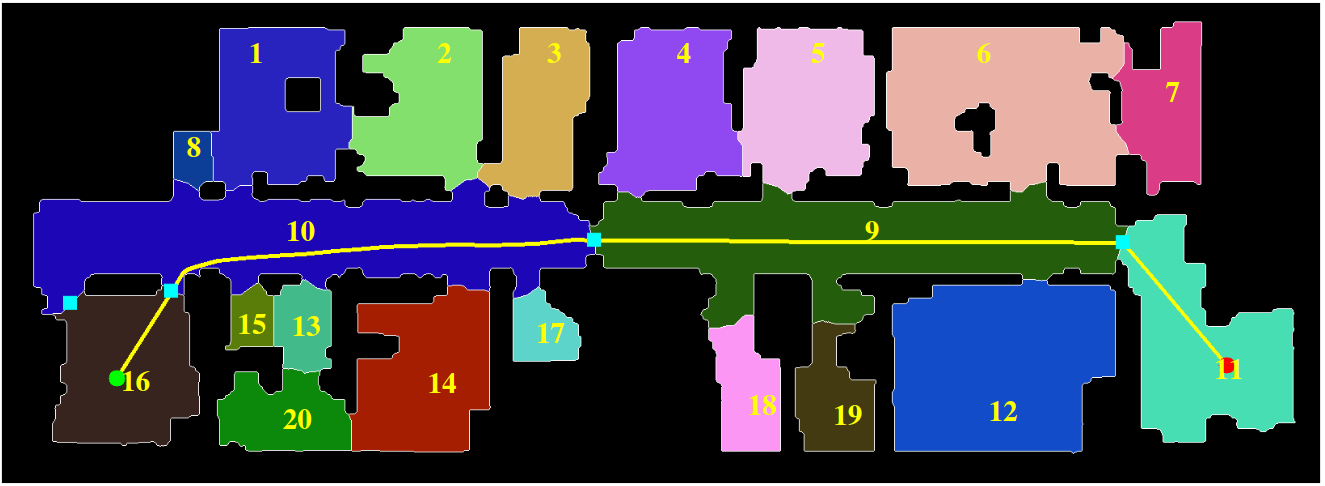
\includegraphics[width=\textwidth]{figures/60_results/ryu_example_path_htm.png}
      \caption{HTM \cite{hou_straight_2021}}
    \end{subfigure}
    \begin{subfigure}{0.75\textwidth}
      \centering
      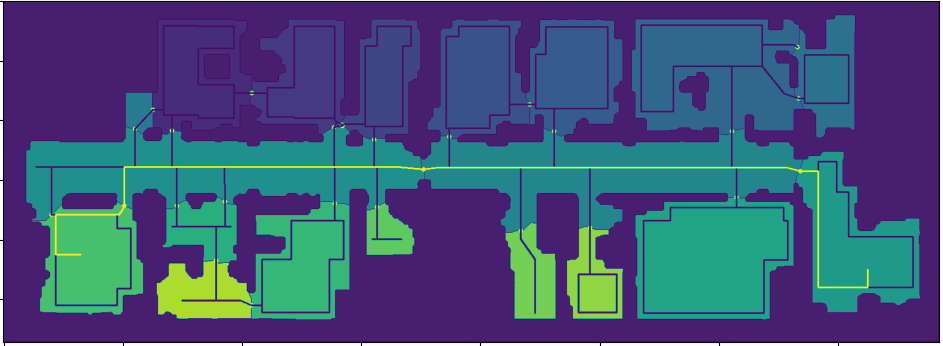
\includegraphics[width=\textwidth]{figures/60_results/ryu_example_path_ilir.png}
      \caption{Hierarchical Planner using ILIR (this work)}
    \end{subfigure}
    \caption[Comparison of hierarchical planning on benchmark map 1]{Comparison of hierarchical planning on benchmark map 1}
    \label{fig:ryu_floor_comparison}
\end{figure}

The proposed hierarchical planner (b) uses the H-Graph to efficiently plan at the room level first and then searches only the corresponding roadmaps of these rooms. Since these roadmaps can be precomputed, a new search can be performed very quickly. In comparison, SIRRT* performs an RRT search in each room for each path. This could also be speeded up by caching the roadmap, but is not described in \cite{ryu_hierarchical_2020}. The problem of choosing the correct room door for connections where two or more doors lead to the same room is solved by both planners. This can be seen in (a) between room 16 and room 10. As well as in (b) on the same rooms. The shortest path inside room 16 would be to connect to the first door on the left, but this would lead to a longer overall path. 

\begin{figure}[h]
    \centering
    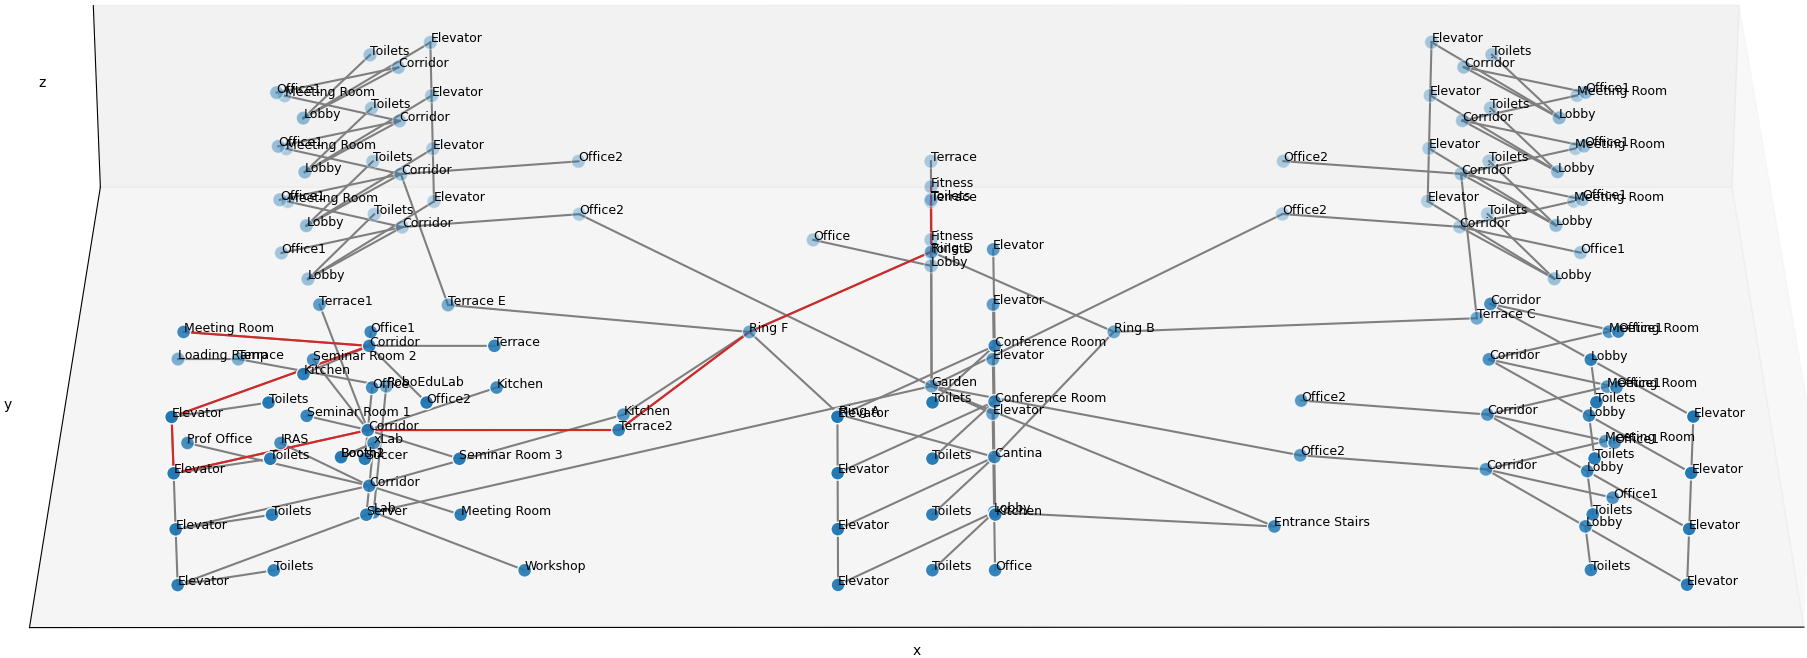
\includegraphics[width=\textwidth]{figures/40_concept/ltc_graph_complete.png}
    \caption[Graph of the IRAS campus for evaluation]{Graph of the IRAS campus for evaluation. All the room level nodes are drawn in the same graph just for visualization.}
    \label{fig:ltc_graph_complete}
\end{figure}

To further test the capabilities of the proposed hierarchical planner, a model of the \gls{iras} research campus is created, see Figure \ref{fig:ltc_graph_complete}. It can be verified that the hierarchical planner is able to plan between arbitrary paths in this complex environment. The built H-Graph has 4 hierarchy levels and a total of 4,454 nodes, the exact number on each hierarchy level can be seen in Table \ref{tab:ltc_graph_nodes}. Note that the total number of nodes on each level includes bridge nodes. Also, the gridmap for each of these rooms has not been recorded. With an estimated average room size of 8x10m, the resulting total number of cells in the gridmaps is 1,672,000 pixels. If all of these cells were searched by a regular planar path planner such as A*, the advantages of the H-Graph and hierarchical planning become obvious.

\begin{table}[ht]
\centering\captionsetup{justification=centering}
\begin{tabular}{ccc}
\hline
\textbf{Level} & \textbf{Name} & \textbf{Number of nodes} \\
\hline
4 & Buildings & 7 \\
3 & Floors & 58\\
2 & Rooms & 209  \\
1 & Nodes on roadmap & 4180  \\
0 & Cells in gridmap & 1,672,000  \\
\hline
\end{tabular}
\caption{Total number of nodes in the H-Graph of the IRAS campus}
\label{tab:ltc_graph_nodes}
\end{table}

%% ==============================
\section{Evaluation in Simulation}
\label{sec:evaluation_simulation}
%% ==============================
To validate the developed concept, it is tested in a simulated hospital environment. The environment was previously presented in Figure \ref{fig:aws_hospital} in Chapter \ref{sec:simulation}. Amazon has made its "AWS RoboMaker Hospital World" \cite{aws_robotics_aws_2023} open source, but has not published any research done with it. This means that it was not possible to compare this approach with related work in the area of multi-floor navigation in the same environment. However, there is a work by Fredriksson et al. \cite{fredriksson_semantic_2023} that uses the same hospital simulation from Amazon, but focuses on detecting semantic features such as intersections and corridors. It also aims to provide a clean roadmap for the robot's global navigation. Figure \ref{fig:aws_comparison} shows a comparison of this approach and the resulting roadmap with the proposed planner and other related work like EVG and RGVG.

\begin{figure}[h]
    \captionsetup[subfigure]{justification=centering}
    \centering
    \begin{subfigure}{.5\textwidth}
      \centering
      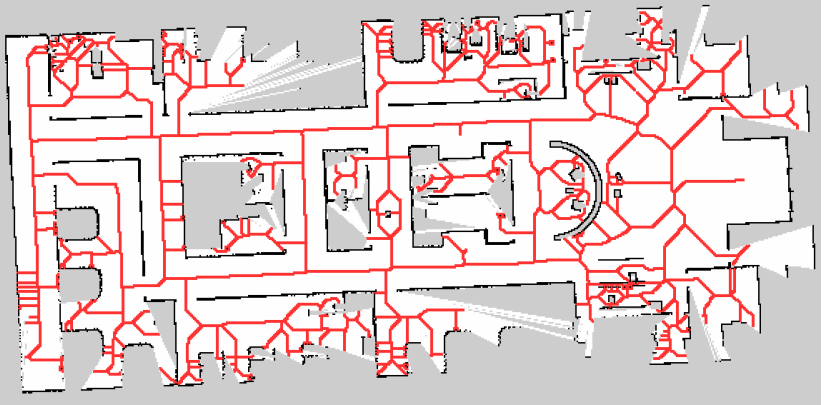
\includegraphics[width=\textwidth]{figures/60_results/aws_roadmap_rgvg.png}
      \caption{RGVG}
    \end{subfigure}%
    \begin{subfigure}{.5\textwidth}
      \centering
      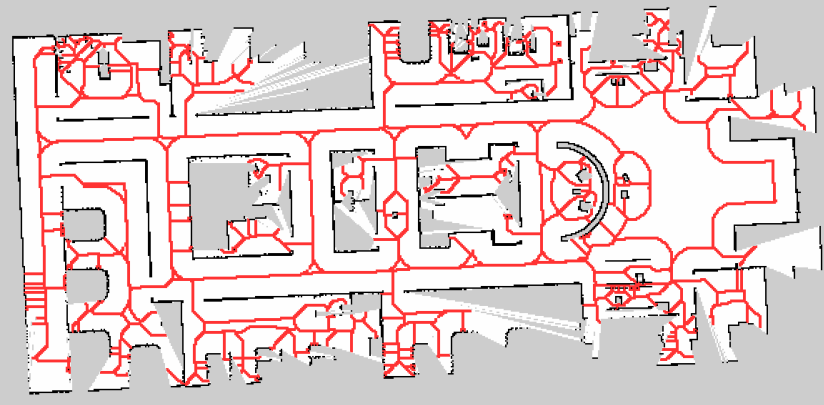
\includegraphics[width=\textwidth]{figures/60_results/aws_roadmap_evg.png}
      \caption{EVG}
    \end{subfigure}
    \begin{subfigure}{.5\textwidth}
      \centering
      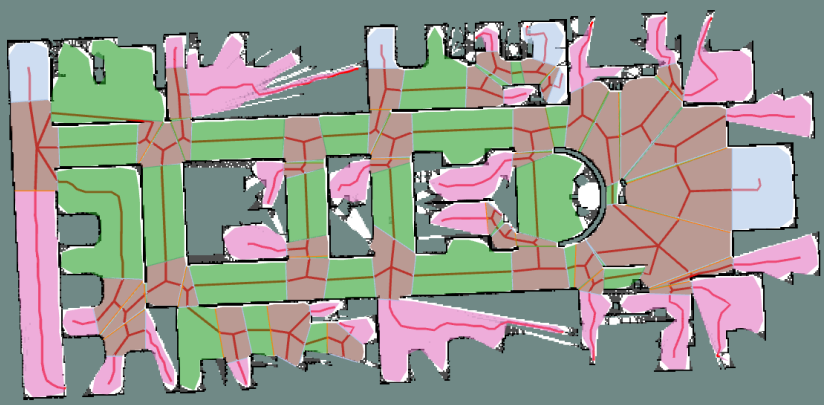
\includegraphics[width=\textwidth]{figures/60_results/aws_roadmap_semantic.png}
      \caption{Semantic \cite{fredriksson_semantic_2023}}
    \end{subfigure}%
    \begin{subfigure}{.5\textwidth}
      \centering
      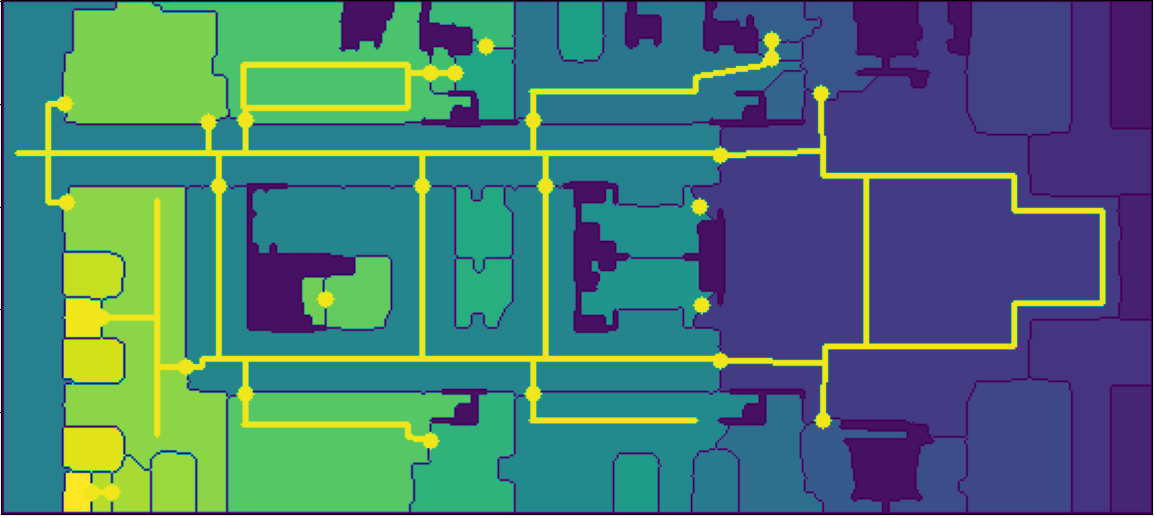
\includegraphics[width=\textwidth]{figures/60_results/aws_roadmap_horizontal.png}\vspace{5pt}
      \caption{ILIR}
    \end{subfigure}
    \caption[Comparison of planning methods for the hospital simulation]{Comparison of planning methods for hospital simulation. For (c), semantic features are colored: Green for paths, brown for intersections, blue for dead ends, and pink for paths to a new frontier. In (d) the segmented rooms are colored with an increasing color palette, the roadmap is yellow.}
    \label{fig:aws_comparison}
\end{figure}

With this roadmap generated by ILIR \ref{fig:aws_comparison} (d), the complete multi-floor navigation with ROS 2 can be tested. Note that the simulation environment has two floors, but they are duplicates of each other with the same layout. Figure \ref{fig:aws_neobotix_simulation} shows the \gls{rviz} (left) and the Gazebo simulation (right). RVIZ represents all the data the robot knows about the environment. It does not matter to the robot if this data comes from a simulation or from sensors in the real world. The robot used in this simulation is the MPO\_500 from Neobotix, because the same planners of this robot are also used in the PeTRA project. The robot can be seen in RVIZ as well as in the lower floor on the left side (the ceiling is transparent). It emits blue rays from the laser scanner just for visualization. The goal for this proof of concept is the elevator on the left. In RVIZ, the path from the hierarchical planner on the ILIR roadmap can be seen as a thin red line. There is also a smaller blue line that represents the current motion of the controller keeping the robot on the path. This is also used to smoothly navigate around the sharp corners in the red roadmap. The goal given by the hierarchical planner is determined by the H-Graph as the shortest path from the bottom floor to the top floor. The location of the elevators on the map was previously marked when the graph was created. When the robot reaches the elevator, it is teleported to the top floor in the simulation and is given a new path to the final goal on the top floor. Once the final goal is reached, another multi-floor navigation with its own behavior tree is triggered to bring the robot back down to the bottom floor. This behavior was successfully tested 10 times in a loop. This proves the capability of the developed multi-floor navigation system.

\begin{figure}[h]
    \centering
    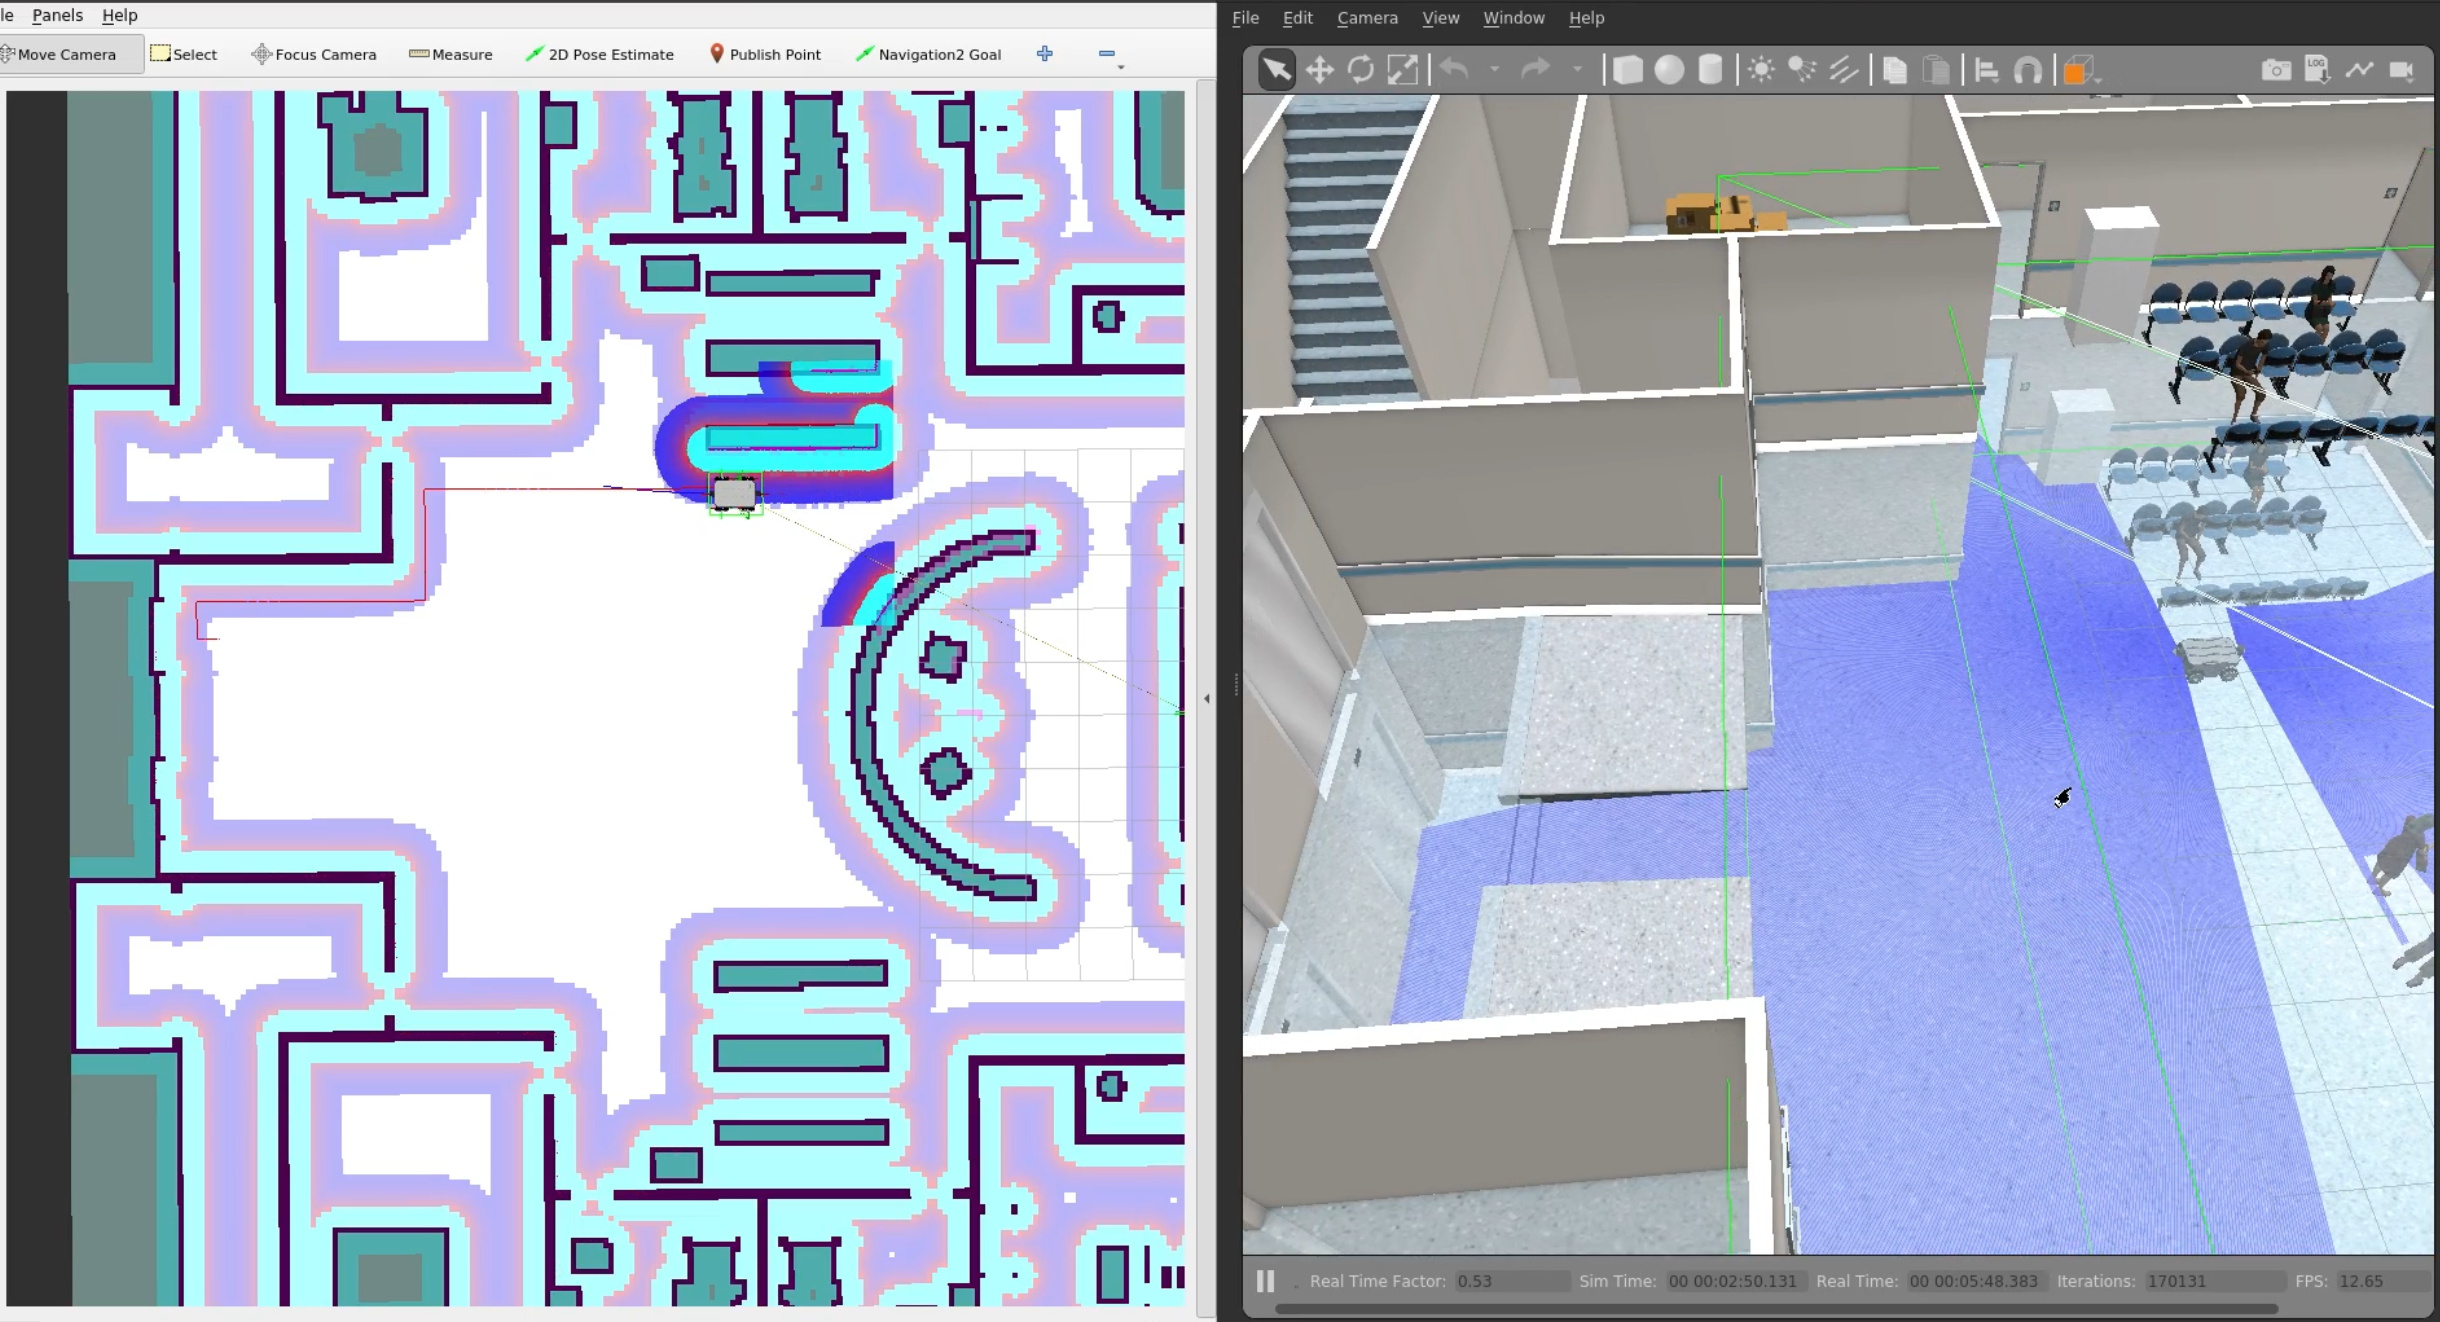
\includegraphics[width=\textwidth]{figures/60_results/aws_neobotix_simulation.png}
    \caption[UML diagram of the H-Graph implementation]{UML diagram of the H-Graph implementation. Blue components were taken from the community, green components were developed in this work.}
    \label{fig:aws_neobotix_simulation}
\end{figure}

Finally the multi-floor navigation system was tested on the real robot. Due to a problem with PeTRA using an old version of the Navigation stack implemented in ROS 1 and the lack of time, not all components can be demonstrated on the real robot. However single components have been tested and work as planned with the current system. This is for example the whole structure of a multi-floor planning request coordinated with the BT.
\begin{figure}[H]
    \centering\captionsetup{justification=centering}
    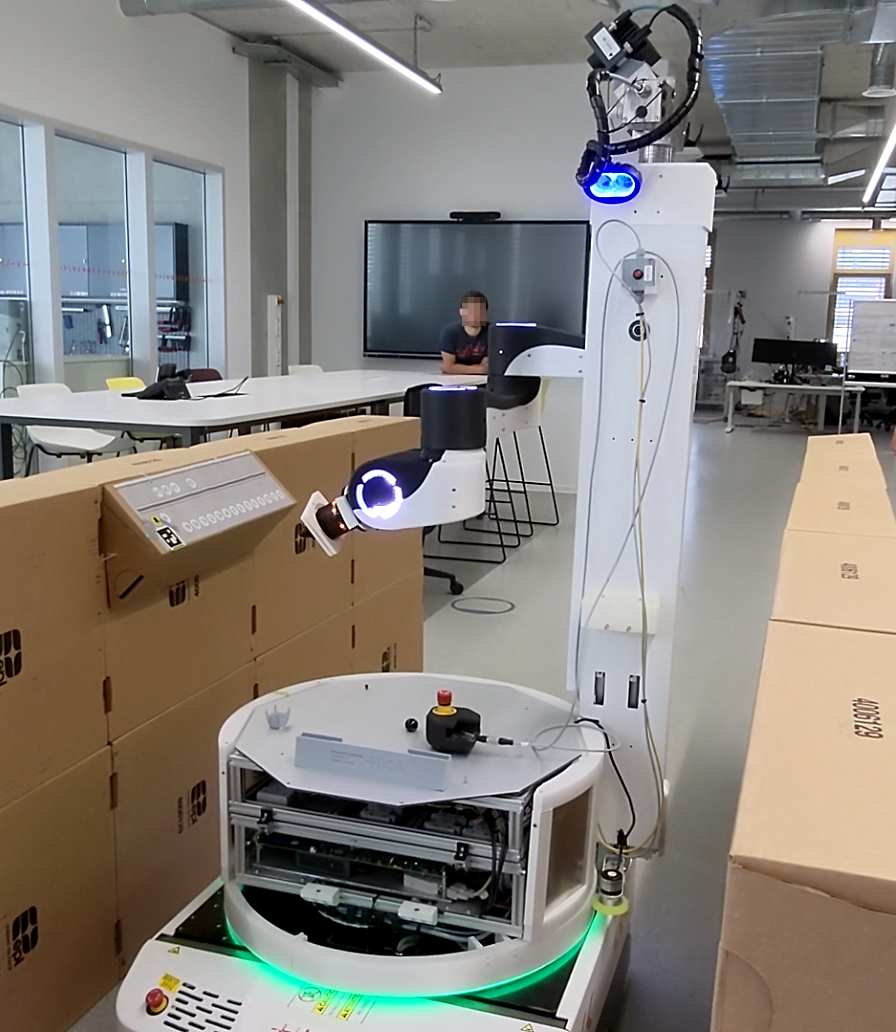
\includegraphics[width=0.6\textwidth]{figures/60_results/petra_elevator.png}
    \caption[The real PeTRA robot in the elevator mock-up]{The real PeTRA robot in the elevator mock-up}
    \label{fig:petra_elevator}
\end{figure}
\noindent
This has been successfully tested and used for navigation in the lab with mock-ups for a potential elevator. A lot of work has also been done in a student project to enable PeTRA to push elevator buttons with its integrated robotic arm. This solves the problem of changing floors where no WLAN interface is available. With these components it was successfully demonstrated that the PeTRA system can perform a multi-floor navigation task in a mock-up environment as shown in Figure \ref{fig:petra_elevator}, where the elevator was simulated by a cardboard box and the floor remained the same. The straight path planner could not be integrated into ROS 1 because it would require a lot of parameter fine-tuning to get the associated path controller to work as expected.
